%\part{Première approche: modèles de vision}
\part{Modèles de vision en Réalité Virtuelle}
	\chapter*{Introduction}
	\addcontentsline{toc}{chapter}{Introduction}
	\markboth{INTRODUCTION}{}
	\par Le terme <<~modèle de vision~>> est très générique et représente en fait un assemblage de briques élémentaires, modulables en fonction des applications et de la finesse du modèle recherchée. Définitions possibles:
	\begin{itemize}
		\item \citep{moreau_traite_2006}: <<~Algorithme qui prend en entrée une image et qui renvoie l'interprétation qu'en fait le système visuel humain.~>>
		\item \citep{pattanaik_multiscale_1998}: <<~Les modèles de vision ont pour objectif de relier la perception visuelle d'un observateur virtuel à la perception visuelle d'un sujet réel regardant un dispositif d'affichage. Le but final étant de caractériser la correspondance visuelle entre la scène virtuelle et l'affichage réel.~>>
	\end{itemize}
	
	\par Un modèle de vision est donc une construction théorique qui vise à reproduire et prédire le fonctionnement de la vision humaine. Le modèle va ainsi intégrer tout un système de modélisation du passage de la lumière dans l'œil, de la captation par la rétine puis du traitement de la lumière par le cerveau. Le modèle de vision est à différencier du prédicateur de vision en cela que ce dernier est inclus, avec d'autres sous-modèles, dans le modèle de vision. Un modèle de vision peut notamment aussi intégrer une prédiction des effets de l'âge mais aussi des comportements plus spécifiques comme le mécanisme d'attention visuelle, ou la reproduction de tons.
	
	\par Nous allons maintenant présenter dans les sections suivantes un état de l'art partiel des modèles de vision, prédicateurs de vision et modèles de reproduction de tons, puis détailler deux modèles particulièrement intéressants:
	\begin{itemize}
		\item Modèle de vision avec vieillissement du système optique \citep{mantiuk_human_2015}.
		\item Prédicateur de vision chromatique complet \citep{pattanaik_multiscale_1998}.
	\end{itemize}
	
	\chapter{État de l'art}
	\par L'état de l'Art ici présenté n'a pas volonté d'être exhaustif sur tous les modèles de vision tant il en existe de types et de variations. On présente néanmoins des classiques ainsi que certaines de leurs ramifications.
	
	\par Si on a défini dans la section précédente le modèle de vision, il reste encore à déterminer les actions et objectifs de deux types de sous-modèles, le Visual Differences Predictor (VDP) et la reproduction de tons:
	\begin{itemize}
		\item La reproduction de tons, ou \textit{tonemapping}, est une technique qui vise à contrebalancer les limites techniques des capteurs d'image par rapport à l'œil humain. En effet, celui ci est -comme on a pu voir précédemment- capable d'intégrer en temps réel un très grand nombre de couleurs et surtout de grands écarts de luminosité, tandis qu'un capteur technologique est (grandement) limité. Le tonemapping est alors une technique pour ramener les informations hors-cadre du capteur dans son champ d'action.
		\item Le VDP est un type d'algorithme qui est amené à donner, objectivement, les différences entre deux traitements d'une même image, par exemple entre l'image initiale et une image après compression. Si le VDP est modélisé sur le système visuel humain, on pourra savoir si les différences entre traitements d'image sont visibles à l'œil nu. Un VDP HDR aura pour objectif de s'assurer que l'interpolation des luminances non-affichables en luminances affichables est efficace.
	\end{itemize}
	
	\par Tout d'abord, il convient de citer les deux modèles fondateurs et sur lesquels la quasi majorité des autres modèles de vision sont adaptés: le \textit{Visual Differences Predictor} de \citep{daly_visible_1992} et le \textit{Visual Discrimination Model} de \citep{lubin_visual_1995}. Si ces deux modèles sont des références absolues, ils restent néanmoins des modèles achromatiques (le traitement et le résultat se font uniquement sur le canal luminance de l'image). Leur équivalent chromatique (traitement sur tous les canaux de l'image, luminance et couleur) est le modèle développé par \citep{pattanaik_multiscale_1998}. Enfin, \citep{rushmeier_comparing_1995} ont formalisé, les premiers, la méthode de reproduction de tons, méthode reprise très largement dans de nombreux modèles par la suite. On en profite également pour pointer vers deux références qui contiennent elle même de très nombreuses références sur le sujet: \citep{moreau_traite_2006} et \citep{bradley_wavelet_1999}.
	
	\section{Modèles principaux dans la littérature}
	\par Le modèle de \citep{daly_visible_1992} est donc un modèle achromatique qui se base sur une simulation de l'adaptation des cellules de la rétine à la luminance. La fonction prend aussi en compte la vision spatiale (c'est à dire la sensibilité aux fréquences spatiales) avec l'intégration de fonctions de sensibilité au contraste. Enfin, le modèle simule aussi les traitement corticaux (c'est à dire la gestion de l'information nerveuse par tout un réseau de neurones) via une fonction dite \textit{cortex}.
		
	\par Parallèlement, le modèle de \citep{lubin_visual_1995} a lui une structure plus logique que le modèle précédent, du point de vue du déroulement de la chaine de vision (de la perception au traitement), néanmoins le traitement se fait toujours de manière achromatique. Il simule l'optique de l'œil et le comportement de la rétine, puis effectue un calcul des contrastes locaux (c'est à dire par zone de l'image perçue) puis il prend en compte l'orientation de l'image et enfin termine par une phase de transduction\footnote{Transducteur. (s.d.). Dans \textit{Dictionnaire Larousse en ligne}. Repéré à \url{http://www.larousse.fr/dictionnaires/francais/transducteur/}}.
	
	\section{Pérennité des modèles principaux}
	\par \citep{lukin_improved_2009} et \citep{bradley_wavelet_1999} ont eu, par rapport au modèle de Daly, des approches radicalement différentes. Le premier a cherché à améliorer la modélisation en complexifiant la fonction de cortex tandis que le second l'a remplacée par une autre approche: une fonction basée sur un modèle en ondelettes.
	Les améliorations de Lukin se concentrent sur une fixation plus précise des seuils utilisés dans la modélisation, l'ajout de la modélisation de l'effet de facilitation pendant l'effet de masque (traitements cognitifs) ainsi que la séparation de l'amplitude et de la phase de la réponse au modèle. L'amplitude servant à calculer le masque de contraste tandis que la phase prend part dans la modélisation de l'effet de facilitation.
	
	\section{Détail des modèles de Mantiuk \textit{et al.}}
	\par Une famille de modèles de vision très intéressante, et basée sur le modèle Daly, est conçue par Rafal Mantiuk et ses collaborateurs: \citep{mantiuk_visible_2004,mantiuk_predicting_2005,mantiuk_human_2015}. Le dernier de ces modèles, qui vient en amélioration des précédents, est d'ailleurs développé en détail par la suite.
	
	\par \citep{mantiuk_visible_2004} proposent un modèle de vision pour les images HDR (High Dynamic Range). Leur hypothèse de base étant que le modèle de Daly est fonctionnel mais reste éloigné de la vision humaine en cela qu'il n'accepte pas une amplitude de luminance suffisante et n'intègre donc pas de mécanisme d'adaptation du système visuel à la luminosité ambiante. Deux modifications principales du modèle initial sont alors opérées:
	\begin{itemize}
	\item Le modèle de Daly part du principe que les photo-récepteurs donnent des réponses égales et subissent des pertes égales quel que soit le niveau de luminance (haut ou bas): une nouvelle transformation de l'information de luminance, cette fois non-linéaire, est proposée.
	\item Une simple fonction de contraste étant insuffisante pour traiter des images avec de grands écarts de luminance, une nouvelle approche est proposée: l'image est filtrée par niveau de luminance puis chaque niveau se voit appliquer une fonction de sensibilité au contraste (CSF).
	\end{itemize}
	
	\par Ensuite, \citep{mantiuk_predicting_2005} apportent une deuxième modification au modèle. La modélisation du passage de la lumière dans l'optique de l'œil est modifiée d'une fonction de diffusion classique (Point Spread Function) au profit d'une fonction de \citep{deeley_simple_1991} (Eq. \ref{eq:deeley_optical_transfer_function}):
	\begin{equation}
	OTF(\rho,d) = \exp \left[ - \left( \frac{\rho}{20.9 - 2.1 \cdot d} \right)^{1.3 - 0.07 \cdot d} \right]
	\label{eq:deeley_optical_transfer_function}
	\end{equation}
	
	\par Avec $\rho$ la fréquence spatiale du stimulus qui traverse l'œil et $d$ le diamètre de la pupille. Ce dernier est quant à lui donné par le modèle de \citep{moon_visual_1944} (Eq. \ref{eq:moon_spencer_pupil_diameter}):
	\begin{equation}
	d = 4.9 - 3 \cdot \tanh \left[ 0.4 \left( \log(Y_{adapt}) + 1.0 \right) \right]
	\label{eq:moon_spencer_pupil_diameter}
	\end{equation}
	
	\par Enfin, \citep{mantiuk_human_2015} apportent une modification fondamentale dans leur modèle, en rajoutant les effets de l'âge de l'observateur simulé sur la perception des erreurs. Ce modèle est largement discuté dans une section suivante (Section \ref{sec:modele_mantiuk}).
	
	\section{Détail des modèles de reproduction de tons}
	\par Après la formalisation de la technique par \citep{rushmeier_comparing_1995}, les algorithmes de reproduction de tons se divisent en trois grandes familles: le traitement des images statiques par des méthodes globales, le traitement des images statiques cette fois ci par des méthodes locales et enfin le traitement des images dynamiques ; \citep{moreau_traite_2006} relèvent un grand nombre de modèles du genre. Cette dernière famille est entièrement revue par \citep{drago_perceptual_2003}.
	
	\par Enfin, \citep{ferwerda_model_1996} proposent un modèle très complet, basé sur le modèle de reproduction de tons lui-même basé sur le coefficient de Ward que l'on a vu précédemment. Ce modèle fonctionne avec des techniques de calcul d'éclairage plus avancées telle que la \textit{Global Illumination}, et ce, à des niveaux de luminosité allant de photopique à scotopique. Sont modélisés: la capture des changements de seuil de visibilité, les changements d'apparence des couleurs, les changements d'acuité visuelle ainsi que la sensibilité à tous ces facteurs au cours du temps. On peut par exemple obtenir toutes les images intermédiaire d'un processus d'adaptation de l'œil à un changement brutal de luminosité, que ce soit du clair vers l'obscur ou inversement (voir Fig. \ref{fig:ferwerda_adaptation_steps}).
	
	\begin{figure}
		\centering
		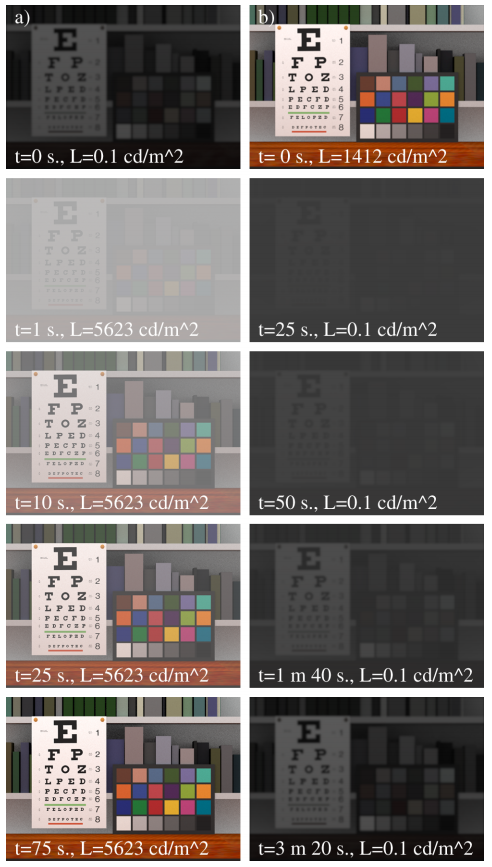
\includegraphics[scale=1]{Figures/FerwerdaAdaptationSteps}
		\caption{Différentes étapes du modèle d'adaptation lumineuse.}{Images tirées de \citep{ferwerda_model_1996}}
		\label{fig:ferwerda_adaptation_steps}
	\end{figure}
	
	\par Nous allons maintenant revenir en détails sur deux modèles particulièrement complets et rigoureux, chacun dans leur domaine: d'un côté le grand mimétisme de la vision humaine et de l'autre la prise en compte avancée des spécificités de l'observateur, et notamment son âge.
	
	\chapter{Modèle de Pattanaik \textit{et al.}}
	\par Le modèle de vision proposé par \citep{pattanaik_multiscale_1998} se positionne face à deux problématiques majeures dans le domaine de l'imagerie informatique: afficher des images ayant un intervalle de luminosité très grand et surtout arriver à afficher des images qui correspondent à une perception similaire à celle de la vision humaine.
	
	\par Il part du principe que beaucoup de modèles ne sont capables de gérer que des informations achromatiques en entrée et font l'impasse sur des caractéristiques plus proches d'une scène naturelle: lumière du jour, amplitude de luminosité étendue, acuité non-uniforme de l'observateur, ...
	
	\par Les auteurs du modèle mettent donc en avant trois points clefs qu'il convient d'utiliser ou d'atteindre dans un modèle de vision:
	\begin{itemize}
	\item des fonctions de sensibilité au contraste (CSFs),
	\item un mécanisme d'adaptation locale de la vision: permet d'améliorer grandement la capacité à voir distinctement dans un intervalle de luminosité très étendu.
	\item un modèle plus élaboré qu'un modèle de seuil: en général, les modèles permettent de définir le seuil en-dessous au au-dessus duquel le visible devient invisible ou inversement. Un modèle plus vaste doit décrire l'intégralité du comportement et non pas uniquement au voisinage du seuil.
	\end{itemize}
	
	\begin{figure}
		\centering
		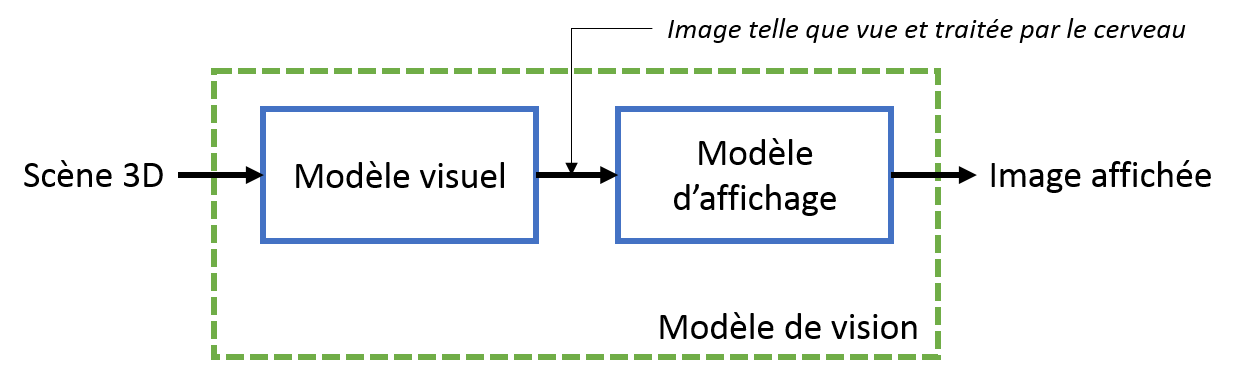
\includegraphics[scale=.75]{Figures/FlowChartPattanaik}
		\caption{Schéma synthétique du déroulé du modèle de \cite{pattanaik_multiscale_1998}}
		\label{fig:flowchart_pattanaik}
	\end{figure}
	
	\par Le modèle proposé est divisé en deux parties principales: le modèle visuel à proprement parler et un modèle d'affichage (voir Fig. \ref{fig:flowchart_pattanaik}). L'algorithme visuel travaille une image d'entrée afin d'en extraire les contrastes des canaux chromatiques et achromatique. Enfin, l'algorithme d'affichage reconstruit une image afin de l'afficher.
	
	\par Le modèle emprunte ses composantes à de nombreux auteurs différents. Il se déroule comme suit (voir Fig. \ref{fig:full_model_pattanaik}):
	\begin{itemize}
		\item Décomposition de l'image via des filtres Gaussiens
		\item Compensation de la dispersion optique dans l'œil, modèle de \citep{westheimer_eye_1986}
		\item Compensation de l'éblouissement, modèle de \citep{spencer_physically-based_1995}
		\item Échantillonnage spectral de tous les étages de la pyramide sauf le plus bas \citep{fairchild_color_1998,wyszecki_color_2000}
		\item Calibration des signaux d'entrée
		\item Traitement spatial des images de chaque canal \citep{burt_laplacian_1983, peli_contrast_1990}
		\item Conversion en canaux chromatiques et achromatique (théorie des processus antagoniques) \citep{hunt_reproduction_1995,fairchild_color_1998}
		\item Passage par des transducteurs de contraste \citep{watson_model_1997}
		\item Combinaison des signaux des cônes et des bâtonnets
		\item Traitement de l'étage de la pyramide restant (le plus bas, qui a été laissé de côté dans la quatrième étape) \citep{fairchild_color_1998}
		\item Résultats du modèle visuel
		\item Reconstruction de l'image par traitement inversé pour l'affichage
	\end{itemize}
	
	\par L'image doit être décomposée à l'aide de filtres gaussiens, de telle manière à ce que les bandes-passantes (ce qui est gardé dans le filtre) correspondent à des fréquences spatiales bien définies: $16$, $8$, $4$, $2$, $1$ et $0.5~cpd$\footnote{cpd: cycles par degrés.}.
	
	\par On réalise ensuite un échantillonnage spectral dans le but de reproduire la réponse des différents cônes et bâtonnets présents dans la rétine. Cet échantillonnage se fait par l'intégration de la distribution de radiance pour chaque pixel après multiplication par l'efficacité lumineuse des photo-récepteurs mis en jeu. L'efficacité pour les cônes est donnée par les courbes de Hunt, Pointer et Estevez \citep{fairchild_color_1998} tandis que l'efficacité des bâtonnets est donnée par l'observateur scotopique de la CIE \citep{wyszecki_color_2000}.
	
	\par Cependant, dans la majeure partie des cas, la valeur de radiance du pixel n'est pas disponible et doit être calculée pour les cônes par une transformation linéaire depuis les valeurs du tri-stimulus CIE 1931 XYZ (Eq. \ref{eq:pattanaik_linear_transform_cones_signal}). Pour les bâtonnets, une approximation est nécessaire, en utilisant l'Eq. \ref{eq:pattanaik_approximation_rods_signal}:
	\begin{equation}
		\left[ \begin{array}{c}L\\ M\\ S\end{array} \right] = \left[ \begin{array}{ccc}
		0.3897 & 0.6890 & -0.0787\\
		-0.2298 & 1.1834 & 0.0464\\
		0 & 0 & 1		
		\end{array} \right] \times \left[ \begin{array}{c}X\\ Y\\ Z\end{array} \right]
		\label{eq:pattanaik_linear_transform_cones_signal}
	\end{equation}
	
	\begin{equation}
		R = -0.702 \cdot X + 1.039 \cdot Y + 0.433 \cdot Z
		\label{eq:pattanaik_approximation_rods_signal}
	\end{equation}
	
	\par Les différents canaux sont ensuite soumis à un traitement spatial, une décomposition en pyramide laplacienne de 7 étages \citep{burt_laplacian_1983}. Les 6 premiers étages sont ensuite convertis en images contrastées \citep{peli_contrast_1990} au moyen d'un gain de luminance (Eq. \ref{eq:pattanaik_laplacian_pyramid_equations}):
	\begin{equation}
		\begin{array}{c}
		G_{cone}(I) = \frac{1}{0.555 \cdot (I+1.0)^{0.85}}\\
		G_{rod}(I) = \left[ \frac{10}{I^2+10} \right] \times \left[ \frac{1}{0.908 \cdot (I+0.001)^{0.85}} \right]
		\end{array}
		\label{eq:pattanaik_laplacian_pyramid_equations}
	\end{equation}
	On obtient au final une image au contraste adapté pour un certain niveau ($ACI_n$ - Image avec contraste adapté au niveau $n$), avec $LP_n$ la réponse au filtre passe-bas de l'image de niveau $n$ ($n$ allant de 1 à 6, en fonction de l'étage de la pyramide concerné) (Eq. \ref{eq:pattanaik_peli_adapted_contrast}):
	\begin{equation}
		ACI_n = G(LP_{n+1}) \times \left[ LP_n - LP_{n+1} \right]
		\label{eq:pattanaik_peli_adapted_contrast}
	\end{equation}
	
	\par Les images contrastées obtenues juste avant, sont ensuite transformées encore, jusqu'au système $AC_1C_2$ qui reprend la Théorie des processus antagoniques, c'est à dire la découpage du traitement de l'image par le cerveau en un canal achromatique ($A$), et deux canaux chromatiques ($C_1$ et $C_2$), voir sections précédentes sur la couleur. La transformation se fait au moyen d'une banale matrice de passage \citep{hunt_reproduction_1995,fairchild_color_1998}:
	\begin{equation}
		\left[ \begin{array}{c}A\\ C_1\\ C_2\end{array} \right] = \left[ \begin{array}{ccc}
		2.0 & 1.0 & 0.05\\
		1.0 & -1.09 & 0.09\\
		0.11 & 0.11 & -0.22		
		\end{array} \right] \times \left[ \begin{array}{c}L\\ M\\ S\end{array} \right]
		\label{eq:pattanaik_linear_transform_lms_to_ac1c2}
	\end{equation}
	
	\par Le signal passe en suite à travers des transducteurs basés sur le contraste pour reproduire la sensibilité au contraste de l'œil. Pour rappel, un transducteur\footnote{Transducteur. (s.d.). Dans \textit{Dictionnaire Larousse en ligne}. Repéré à \url{http://www.larousse.fr/dictionnaires/francais/transducteur/}} est une fonction ou un mécanisme qui permet de transformer une grandeur en une autre, comme par exemple un mouvement en électricité ou une lumière en électricité. Les transducteurs sont ici utilisés pour supprimer de l'image le contraste qui serait imperceptible dans les conditions (d'éclairage) données. Leurs valeurs sont limitées à 50 pour reproduire les limitations en luminosité du système visuel. Les auteurs du modèle utilisent les équations de \citep{watson_model_1997} modifiées pour être inversibles (Eq. \ref{eq:pattanaik_transducers}):
	\begin{equation}
	\begin{array}{c}
	
	T_{cone,achromatic}(c) = \begin{cases}
	22.4 \cdot \sqrt{\frac{c}{0.536}} & \mbox{si } c \geq 0.536\\
	22.4 \cdot \left( \frac{c}{0.536} \right)^p & sinon
	\end{cases}\\
	
	T_{cone,chromatic}(c) = \begin{cases}
	22.4 \cdot \sqrt{\frac{c}{0.176}} & \mbox{si } c \geq 0.176\\
	22.4 \cdot \left( \frac{c}{0.176} \right)^p & sinon
	\end{cases}\\
	
	T_{rod}(c) = \begin{cases}
	22.4 \cdot \sqrt{\frac{c}{0.0335}} & \mbox{si } c \geq 0.0335\\
	22.4 \cdot \left( \frac{c}{0.0335} \right)^p & sinon
	\end{cases}
	
	\end{array}
	\label{eq:pattanaik_transducers}
	\end{equation}
	
	\par Les valeurs de p sont données dans la Table \ref{tab:pattanaik_transducers_p_values}.
	
	\begin{table}
		\centering
		\label{tab:pattanaik_transducers_p_values}
		\small
		\begin{tabular}{|l|l|l|l|l|l|l|}
			\hline
			\textbf{Fréquence spatiale (cpd)} & \textbf{0.5} & \textbf{1.0} & \textbf{2.0} & \textbf{4.0} & \textbf{8.0} & \textbf{16.0}\\
			\hline
			\hline	
			\textbf{p (achromatique)} & 1.93 & 1.35 & 1.15 & 1.04 & 1.15 & 1.40\\
			\hline
			\textbf{p (chromatique)} & 1.93 & 1.93 & 2.35 & 2.85 & - & -\\
			\hline
			\textbf{p (bâtonnets)} & 3.39 & 3.39 & 4.50 & 7.64 & - & -\\
			\hline
		\end{tabular}
		\caption{Valeurs de la puissance dans les fonctions de transducteurs de \citep{watson_model_1997}}
	\end{table}
	
	\par Le canal chromatique final est en fait une combinaison des valeurs de la composante A des tri-stimulus des cônes et des bâtonnets. Le calcul se fait au moyen de l'Eq. \ref{eq:pattanaik_combination_rodes_cones}. La valeur $7$ est obtenue par calibration:
	\begin{equation}
		A_{total} = A_{cones} + \frac{A_{batonnets}}{7}
		\label{eq:pattanaik_combination_rodes_cones}
	\end{equation}
	
	\par Cette étape conclue le traitement des 6 premiers étages de la pyramide de décomposition.
	
	\par Après quoi, le traitement du dernier et septième étage de la pyramide se fait via des transducteurs passe bas (Eq. \ref{eq:pattanaik_lowpass_transducers}) \citep{fairchild_color_1998}:
	\begin{equation}
		\begin{cases}
			T_{LP,cones,achromatique}(LP) = 30.5 \cdot \sqrt{LP}\\
			T_{LP,cones,chromatique}(LP) = 53.3 \cdot \sqrt{LP}\\
			T_{LP,batonnets}(LP) = 122 \cdot \sqrt{LP}\\
		\end{cases}
		\label{eq:pattanaik_lowpass_transducers}
	\end{equation}
	
	\par Au point intermédiaire, à l'issue du modèle visuel, on obtient donc les résultats suivants:
	\begin{itemize}
		\item 1 canal achromatique
		\item 2 canaux chromatiques
		\item 6 images issues d'un filtre spatial bande-passante
		\item 1 image issue d'un filtre passe-bas
	\end{itemize}
	
	\par Enfin, on effectue le processus de reconstruction de l'image en faisant un traitement étape-par-étape inverse par rapport au modèle visuel de manière à recréer le signal perçu par les cônes pour l'afficher. On prend les fonctions inverses des transducteurs évoqués précédemment (Eq. \ref{eq:pattanaik_lowpass_transducers}). On passe d'une décomposition de la lumière en mode chromatique/achromatique ($AC_1C_2$) au découpage reproduisant le fonctionnement des cônes et bâtonnets ($LMS$), en utilisant la matrice inverse et enfin on applique un mécanisme de gain inverse en fonction des conditions d'affichage. Pour finir, on effectue la dernière transformation en allant de $LMS$ à l'espace colorimétrique adapté au moyen d'affichage (CIECAM, CIELAB, CIELUV, RGB, ...).
	
	\begin{figure}
		\centering
		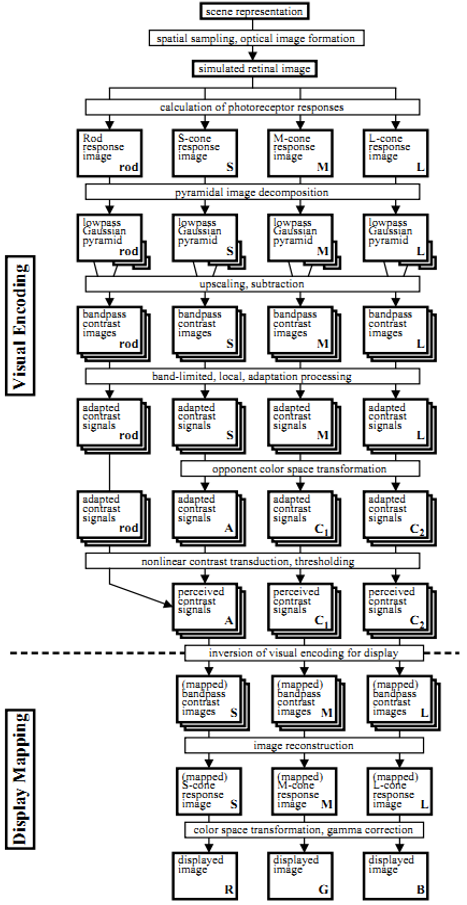
\includegraphics[scale=1.25]{Figures/PattanaikFullModel}
		\caption{Schéma exhaustif du traitement de l'image par le modèle de \cite{pattanaik_multiscale_1998}}
		\label{fig:full_model_pattanaik}
	\end{figure}
	
	\par En conclusion, \citep{pattanaik_multiscale_1998} ont mis sur pied un modèle extrêmement précis et pertinent, composé de sous-modèles disponibles dans la littérature. Cependant, ce modèle est statique, c'est à dire qu'il ne prend pas en compte la composante temporelle et ne fonctionne que pour traiter une image seule, et non pas intégré dans une boucle de calcul d'image en temps réel. Nous allons maintenant aborder le modèle de \citep{mantiuk_human_2015}.
	
	\chapter{Modèle de Mantiuk \& Ramponi}
	\label{sec:modele_mantiuk}
	\par Comme on a pu voir précédemment, l'âge de l'observateur peut avoir une grande influence sur un certain nombre de paramètres dans la vision ; tant de manière physiologique que cognitive. Cependant, le modèle que nous présentons ici, celui de \citep{mantiuk_human_2015}, est basé sur un prédicateur nommé HDR-VDP-2 et amélioré selon quatre grands axes: le vieillissement du cristallin, la réduction du diamètre de la pupille avec l'âge, les éblouissement invalidants et une composante de dégradation cognitive. 
	
	\par La contribution la plus importante à la dégradation de la vision au cours du temps vient du vieillissement du cristallin. La lentille continue de grossir et de générer des nouvelles fibres, compressant et accumulant ainsi les fibres plus anciennes dans la région centrale du cristallin. Celui-ci devient donc de plus en plus rigide et de moins en moins transparent.
	
	\par Le cristallin est modélisé comme un filtre optique dépendent de la longueur d'onde et qui réduit la quantité de lumière que la rétine reçoit. Cependant ce filtre a peu d'effet en vision photopique (vision de jour) et est plus efficace en dessous de $3~cd/m^2$, c'est à dire dans les domaines mésopique et scotopique.
	\citep{mantiuk_human_2015} reprennent ici le modèle de \citep{pokorny_aging_1987}. pour le vieillissement du cristallin (Eq. \ref{eq:vieillissement_cristallin}):
	\begin{equation}
		O_D(a) = \begin{cases}
			 L_1 \cdot (1+0.02 \cdot (a-32))+L_2 & a \leq 60 \\ L_1 \cdot (1.56+0.0667 \cdot (a-60))+L_2 & a \geq 60 \end{cases}
		\label{eq:vieillissement_cristallin}
	\end{equation}
	
	\par Avec $O_D$ la densité optique du cristallin, $a$ l'âge du sujet et $L_1$, $L_2$ des constantes issues de tables dans le modèle de Porkony \textit{et al.}.
	
	
	\par \citep{mantiuk_human_2015} incluent aussi dans leur modèle un mécanisme d'efficacité lumineuse (valable seulement dans le domaine photopique) qui fut validé et entériné par la CIE en 1924. Les résultats liés à ce modèle sont disponibles chez \citep{sagawa_spectral_2001}.
	
	\par L'éblouissement (ou \textit{Sensibility Glare} en anglais) est une pollution lumineuse qui intervient en présence de lumière très vive directement dans le champ de vision. Cette pollution atténue les hautes fréquences spatiales et réduit le contraste perçu sur la rétine. La prise en compte de la sensibilité à l'éblouissement en fonction de l'âge est elle aussi étayée par un modèle de la CIE: \citep{vos_cie_1999}.
	
	\par Le diamètre pupillaire moyen tend à diminuer avec l'âge, on parle alors de \textit{myosis} (l'effet contraire étant la \textit{mydriase}). Ce phénomène a été modélisé par un grand nombre de chercheurs différents ; \citep{watson_unified_2012} proposent à la fois une revue des différents modèles mais surtout un modèle unifié pour l'évolution du diamètre de la pupille. C'est ce modèle qui est utilisé dans le modèle de vision avec vieillissement de l'œil de \citep{mantiuk_human_2015}.
	
	\par Le modèle est le suivant (Eq. \ref{eq:diam_pupille_aging}):
	\begin{equation}
		\begin{cases}
		S(l,a,f) = (a-28.58) \times (0.02132-0.009562 \cdot D_{SD})\\
		D_{SD} = 7.75 - \frac{5.75 \times k}{k+2}\\
		k = \left( \frac{L \times f}{846} \right)^{0.41}
		\end{cases}
		\label{eq:diam_pupille_aging}
	\end{equation}
	
	\par Avec $S$ le diamètre pupillaire, $a$ l'âge de l'individu, $L$ le niveau de luminosité auquel l'œil est adapté (en $cd/m^2$) et $f$ la zone de champ.
	
	\par Ensuite, \citep{burton_aging_1993} ont mesuré la perte de sensibilité causée par l'affectation des récepteurs et des processus cognitifs entre des jeunes adultes et des personnes âgées. Ces mesures ont été réalisées avec un laser permettant d'ignorer le système optique et d'envoyer directement une image sur la rétine. Les résultats donnent de légères variations entre les populations d'âge différent. \citep{mantiuk_human_2015} proposent alors leur propre modèle empirique (Eq. \ref{eq:neural_component_model_mantiuk}):
	\begin{equation}
		log_{10}(\Delta S) = - (\beta \times log_2(\rho + a)) \times max(a-24;0)
		\label{eq:neural_component_model_mantiuk}
	\end{equation}
	
	\par Avec $a$ l'âge du sujet, $\rho$ la fréquence spatiale du stimulus (en $cpd$). $\alpha = 0.75$ et $\beta = 0.00195$ sont des valeurs empiriques proposées par les auteurs du modèle.
	
	\par Enfin, cette modélisation est toutefois à prendre avec recul car un grand nombre de valeurs utilisées ici ont été mesurées pendant des expérimentations réalisées sur des écrans CRT (Cathodiques) ayant un spectre de luminosité assez réduit (de $0.1$ à $80~cd/m^2$).
	
	\chapter*{Conclusion}
	\addcontentsline{toc}{chapter}{Conclusion}
	\markboth{CONCLUSION}{}
	\par L'étude des modèles de visions et leurs traductions vers le domaine de l'informatique semble être un domaine déjà fortement décrit et bien maitrisé. Une contribution directe dans ce domaine n'est alors ni très évidente ni très pertinente. On pourrait éventuellement tenter d'appliquer le modèle de Pattanaik \textit{et al.} en temps réel mais la portée scientifique semble limitée. On décide alors de laisser cette approche de côté pour en prendre une nouvelle.
	
	\par Plutôt que de s'intéresser à une capture d'image respectant le même processus que la vision humaine, on se penche sur un autre aspect jouant un rôle prépondérant dans le réalisme: l'affichage correct de ce qui a été capturé dans la scène 3D. En effet, si une fois l'image capturée proprement (via une mise en place du modèle de Pattanaik \textit{et al.} par exemple), si le système n'est pas capable de restituer l'image dans la même gamme de perception que celle de l'œil humain, le réalisme vis à vis de l'utilisateur sera amoindri.
	
	\par On propose alors, non pas de développer un modèle d'affichage, mais une méthode pour quantifier la qualité du système d'affichage immersif, en fonction de la modélisation du système visuel humain.